\section{Behaviour at criticality}

\begin{figure*}[h!]
    \centering
    \setlength{\tabcolsep}{2pt}
    \begin{minipage}[t]{0.48\textwidth}
        \centering
        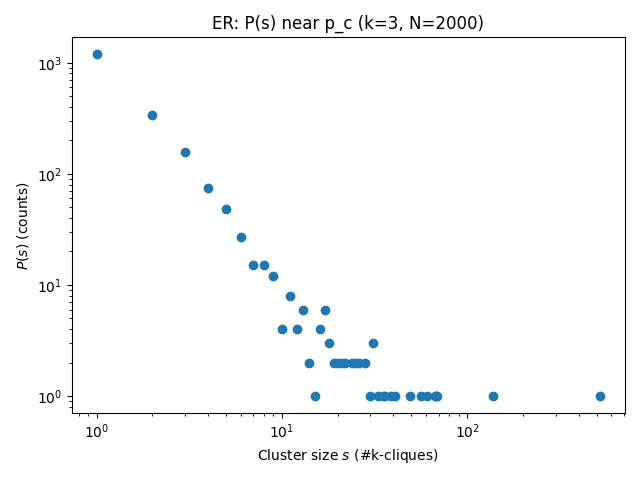
\includegraphics[width=\textwidth]{images/IMAGES TASK2/ER_Ps_k3_N2000.png}
        \subcaption{$P(s)$ distribution for $k=3$, $N=2000$.}
        \label{fig:Ps_k3}
    \end{minipage}
    \hfill
    \begin{minipage}[t]{0.48\textwidth}
        \centering
        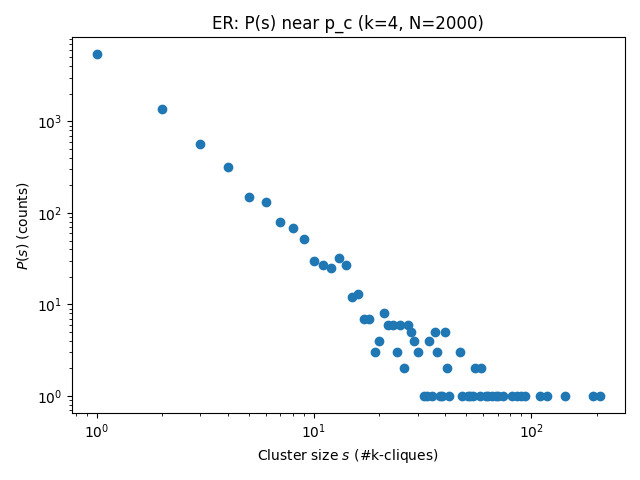
\includegraphics[width=\textwidth]{images/IMAGES TASK2/ER_Ps_k4_N2000.png}
        \subcaption{$P(s)$ distribution for $k=4$, $N=2000$.}
        \label{fig:Ps_k4}
    \end{minipage}
    \caption{Cluster size distributions $P(s)$ in ER graphs at criticality. 
    For $k=3$ the distribution decays rapidly, while for $k=4$ the tail is more extended, 
    with rare but larger clusters.}
    \label{fig:Ps_ER}
\end{figure*}

Considering the cluster size distribution at the critical point, it shows that it behaves differently depending on k:

- For $k=3$ (Fig.~\ref{fig:Ps_k3}), $P(s)$ decays steeply and large clusters 
  are essentially absent beyond a certain value. 
  This indicates critical fluctuations typical of a continuous transition, 
  but the range of accessible cluster sizes is relatively narrow.  

- For $k=4$ (Fig.~\ref{fig:Ps_k4}), the distribution extends further: 
  although large clusters are rare, they appear up to $s > 100$. 
  This heavier tail reflects that, in finite systems, clique percolation 
  with $k \geq 4$ can still generate sizeable clusters near criticality, 
  even though theory predicts that the giant component vanishes in the 
  thermodynamic limit.  

Thus (Fig.~\ref{fig:Ps_ER}), $k=3$ shows a continuous transition with limited 
cluster range, while $k=4$ displays rarer but larger clusters, consistent 
with finite-size effects and the theoretical expectation that the giant 
component disappears as $N \to \infty$.

\begin{figure*}[h!]
    \centering
    \setlength{\tabcolsep}{2pt}
    \begin{minipage}[t]{0.48\textwidth}
        \centering
        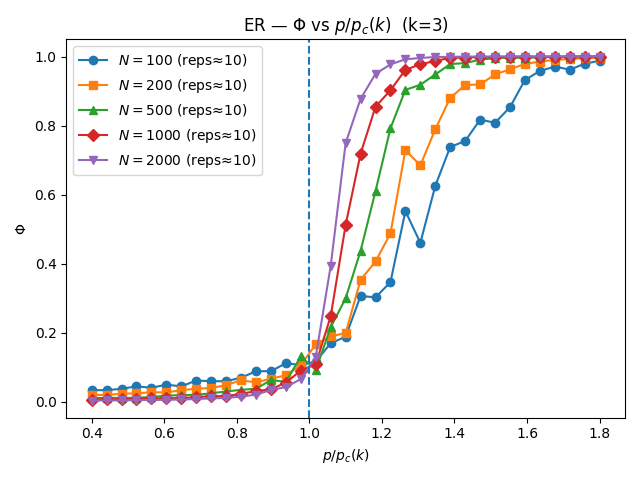
\includegraphics[width=\textwidth]{images/IMAGES TASK2/ER_phi_k3.png}
        \subcaption{Order parameter $\phi_k$ for $k=3$.}
        \label{fig:phi_k3}
    \end{minipage}
    \hfill
    \begin{minipage}[t]{0.48\textwidth}
        \centering
        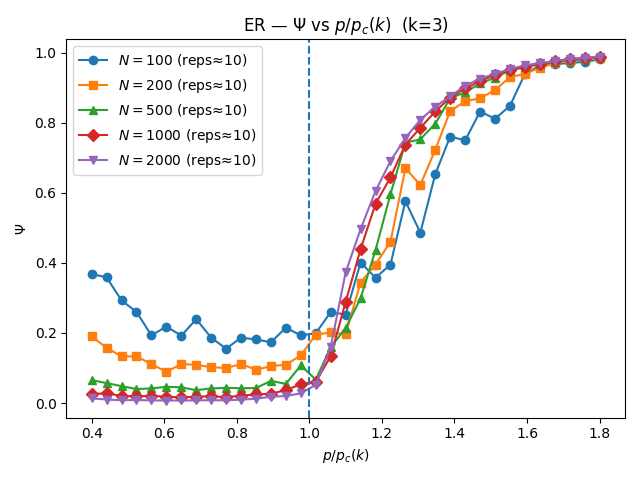
\includegraphics[width=\textwidth]{images/IMAGES TASK2/ER_psi_k3.png}
        \subcaption{Order parameter $\psi$ for $k=3$.}
        \label{fig:psi_k3}
    \end{minipage}
    \caption{Order parameters for $k=3$. 
    Both $\phi_k$ (left) and $\psi$ (right) increase smoothly with $p$, 
    showing consistent finite-size scaling and confirming a continuous transition.}
    \label{fig:orderparam_k3}
\end{figure*}

\section{Other simulations}
Considering the case $k=3$ (Fig.~\ref{fig:orderparam_k3}):
\begin{itemize}

\item $\phi_k$}
For $p/p_c(k) < 1$ we have $\phi_k \approx 0$, indicating the absence of a giant clique component. 
Around $p/p_c(k) \simeq 1$ the parameter increases rapidly, with a sharper transition as $N$ grows. 
For small $N$ values, smoothing and finite-size fluctuations appear. 
This behavior is consistent with a continuous (second-order) transition.

\item $\psi$}
Below the threshold $\psi$ remains very small, especially for large $N$, indicating fragmented cliques. 
Beyond the critical point it increases regularly, showing the emergence of a large-scale interconnected structure. 
For large $N$, the curves collapse onto each other, confirming finite-size scaling.
\end{itemize}
As for $k=4$ they reveal a continuous transition at $p/p_c(k)=1$ in the clique space and discontinuous transition in the vertex. 
The simulations exhibit finite-size scaling effects that vanish as $N$ increases, in agreement with the theoretical predictions of clique percolation.


\section{Erdős–Rényi Baseline}
The Erdős–Rényi random graph $G(N,p)$ is defined on $N$ nodes, where each possible edge 
is included independently with probability $p$. Varying $p$ directly controls the average 
degree of the network,
\begin{equation}
    \langle k \rangle = p(N-1) \simeq pN,
\end{equation}
making ER graphs particularly convenient for percolation studies.  
By simply tuning $p$, one generates ensembles of graphs with different expected connectivities, 
a feature more direct than in scale-free or small-world models.

A giant connected component emerges once the average degree exceeds unity, yielding the 
percolation threshold
\begin{equation}
    p_c = \frac{1}{N}.
\end{equation}
At criticality, the fraction $S$ of nodes in the largest connected component satisfies
\begin{equation}
    S = 1 - e^{-\langle k \rangle S}.
\end{equation}

This provides the natural baseline: $k=2$ clique percolation is exactly equivalent to 
classical ER percolation, while $k \geq 3$ introduces genuinely higher–order phenomena.

\begin{figure}[H]
    \centering
    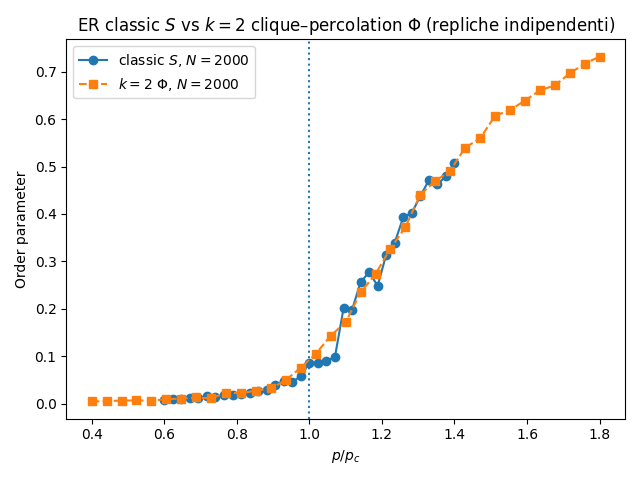
\includegraphics[width=0.55\linewidth]{images/IMAGES TASK2/ER_classic_vs_k2_N2000.png}
    \caption{Comparison between classical percolation ($S$) and $k=2$ clique percolation 
    ($\Phi$) in an ER graph with $N=2000$. The two curves overlap, confirming their equivalence.}
    \label{fig:ER_k2}
\end{figure}

As shown in Fig.~\ref{fig:ER_k2}, the order parameter $S$ of classical ER percolation and 
$\Phi$ for $k=2$ clique percolation coincide perfectly, validating that clique percolation 
reduces to the classical case when $k=2$.\\
The missing points of classical ER percolation were not simulated outside of the range $[0.6, 1.4]$
